\documentclass[smallextended]{svjour3}
\usepackage{fix-cm}
\usepackage[T1]{fontenc}
\usepackage[utf8]{inputenc}
\usepackage{mathptmx}
\usepackage{amsmath,amssymb,graphicx,booktabs,tabularx,url}
\usepackage{placeins}
\usepackage[numbers,sort&compress]{natbib}
\usepackage[hidelinks]{hyperref}
\journalname{Computing}
\smartqed
\setlength{\emergencystretch}{2em}
\newcommand{\CollegePRDelta}{-0.90780}
\newcommand{\CollegePRLoss}{9.01}
\newcommand{\CollegePRSaving}{86.44}
\newcommand{\CollegePRfiveDelta}{-0.43094}
\newcommand{\CollegePRfiveLoss}{4.28}
\newcommand{\CollegePRfiveSaving}{82.83}
\newcommand{\CollegeDegreeDelta}{0.00000}
\newcommand{\CollegeDegreeLoss}{0.00}
\newcommand{\CollegeDegreeSaving}{86.59}
\newcommand{\GrqcPRDelta}{-0.25082}
\newcommand{\GrqcPRLoss}{5.07}
\newcommand{\GrqcPRSaving}{92.70}
\newcommand{\GrqcPRfiveDelta}{0.00000}
\newcommand{\GrqcPRfiveLoss}{0.00}
\newcommand{\GrqcPRfiveSaving}{88.14}
\newcommand{\GrqcDegreeDelta}{0.00000}
\newcommand{\GrqcDegreeLoss}{0.00}
\newcommand{\GrqcDegreeSaving}{92.77}
\newcommand{\WikiPRDelta}{-40.69334}
\newcommand{\WikiPRLoss}{73.01}
\newcommand{\WikiPRSaving}{96.42}
\newcommand{\WikiPRfiveDelta}{-13.53012}
\newcommand{\WikiPRfiveLoss}{24.28}
\newcommand{\WikiPRfiveSaving}{91.98}
\newcommand{\WikiDegreeDelta}{0.00000}
\newcommand{\WikiDegreeLoss}{0.00}
\newcommand{\WikiDegreeSaving}{96.26}

\begin{document}
\title{Reference Budgets and Ranking Precision in Candidate-Restricted Influence Maximization}
\titlerunning{Reference budgets and ranking precision}
\author{\mbox{Jiayue Sun} \and \mbox{Binbin Yong} \and \mbox{Junjie An} \and \mbox{Tianyu Bo} \and \mbox{Shuai Li}}
\authorrunning{Jiayue Sun et al.}
\institute{Jiayue Sun \at School of Artificial Intelligence, Lanzhou University, Lanzhou 730000, China
\and Binbin Yong (corresponding author) \at School of Information Science and Engineering, Lanzhou University, Lanzhou 730000, China \\
\email{yongbb14@lzu.edu.cn}
\and Junjie An, Tianyu Bo and Shuai Li \at Lanzhou University, Lanzhou, China}
\date{}
\maketitle
\begin{abstract}
Candidate restriction can reduce influence-maximization search costs, yet its apparent quality depends on a reference solution that is itself estimated. A measured gain or loss may reflect reference sampling, numerical changes in candidate eligibility, or both. We use paired selection and independent spread evaluation to distinguish these effects by varying reference budget and ranking precision separately. Evidence comes from a small, selected sample of real-world networks: three external topologies, with four small contact graphs providing separate controls. On ca-GrQc, increasing the reference budget changes mean incremental spread from a 5.61\% gain to a 5.07\% loss. This reversal disappears in a post-hoc control that tightens PageRank tolerance. Budget-dependent seed changes persist, and reference-set changes have different utility consequences. Across the external networks, degree-based pools reproduce all 15 highest-budget reference trajectories, whereas PageRank losses persist on the two directed networks. These findings identify how numerical choices can alter judgments of candidate restriction. Reporting candidate-pool stability and independently evaluated spread alongside reference agreement makes the basis of a measured quality--cost trade-off explicit.
\keywords{influence maximization \and Monte Carlo simulation \and candidate restriction \and evaluation methodology \and reproducibility}
\end{abstract}

\section{Introduction}
Influence maximization selects a limited set of seed vertices to maximize expected spread under a specified diffusion model \cite{ref1}. It formalizes targeted seeding, such as choosing initial adopters in a social network. Greedy selection repeatedly estimates the spread gained by adding a vertex, making computational cost a central concern. Lazy evaluation, reuse of sampled realizations and sampling-based optimization address this cost through different computational strategies \cite{ref7,ref8,ref2}. Candidate restriction reduces the set of vertices eligible for selection. Its practical value depends on how much spread is retained for the computation saved.

Establishing this trade-off is difficult when the full-candidate reference is itself selected from finitely sampled diffusion worlds. The observed gap compares two computed seed sets, and its interpretation depends on how both were obtained. Misattributing that gap can lead to an incorrect judgment about whether a cheaper candidate pool preserves the reference's utility.

Reference sampling and candidate ranking enter this comparison at different stages. Increasing the sampling budget can change the full-reference seeds and the measured gap to a restricted method. Ranking precision acts before greedy selection, where small score changes can exchange vertices at the candidate-pool boundary. A change in the apparent quality of a restricted method may therefore depend on either numerical choice. Seed disagreement alone cannot resolve this ambiguity because different sets can have similar independently evaluated spread.

We address this evaluation problem by separating the construction of the reference, the construction of the candidate pool and the assessment of selected seeds. The analysis asks whether an apparent budget effect survives a ranking-precision control and how reference-set changes translate into spread differences. Full and restricted selection share the propagation graph, sampled-world prefix and tie rule (Fig.~\ref{fig:evaluation-mechanism}). Independent evaluation then measures their paired utility difference. This design makes each comparison explicit while keeping seed eligibility as the only difference between the two selection arms.

The evidence is drawn from a small, selected sample of real-world networks. Three external communication, collaboration and voting topologies test the transfer of earlier findings from four small contact graphs. The contact-graph results provide separate budget, propagation-parameter and coupling controls. A post-hoc PageRank analysis tests whether the external budget comparison depends on solver tolerance.

The main contributions are:
\begin{enumerate}
\item[(1)] \textbf{Ranking precision changes the interpretation of an apparent budget effect.} On ca-GrQc, tightening PageRank tolerance exchanges two of 20 candidates. The default mean gain-to-loss reversal then disappears, although budget-dependent seed changes remain. This post-hoc control shows that the reversal cannot be interpreted as a reference-budget effect independent of ranking precision.
\item[(2)] \textbf{Reference-set instability can accompany a small average spread improvement.} Increasing $W$ from 1280 to 5120 changes 16 of 40 contact-graph reference sets. The mean independently evaluated spread increase is 0.01111 nodes across all 40 network--path pairs. These measurements distinguish the frequency of seed-set changes from the magnitude of the resulting utility changes.
\item[(3)] \textbf{Degree and PageRank agreement diverge on the external networks.} At $W=1280$, Degree-4k reproduces all 15 full-reference trajectories using 20 candidates and less selection time in this implementation. Default PageRank-4k reproduces none; losses on CollegeMsg and wiki-Vote persist under tighter tolerance. The comparison identifies limits to the earlier contact-graph agreement and ties the observed cost savings to preservation of the tested reference.
\end{enumerate}

\begin{figure}[t]
\centering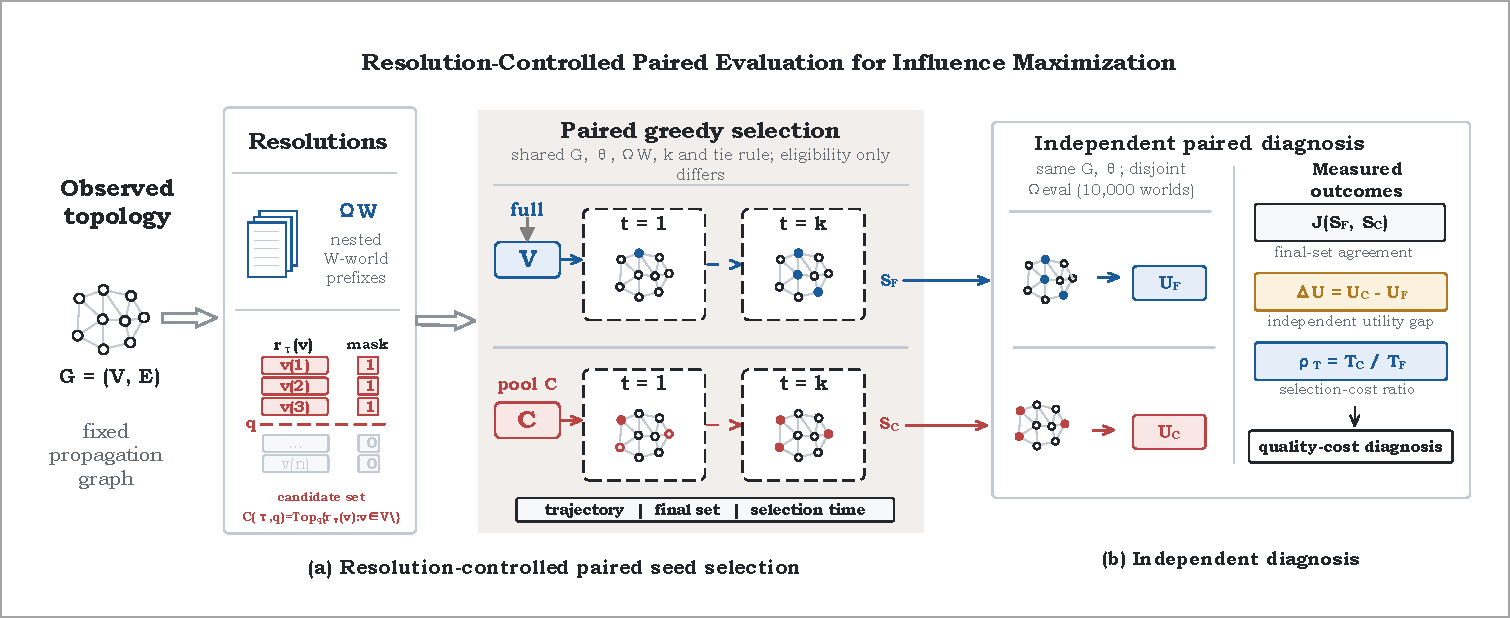
\includegraphics[width=\linewidth]{FigEvaluationMechanism.pdf}
\caption{Paired evaluation separates reference resolution, ranking resolution and restriction quality. (a) The selection budget $W$ and ranking tolerance $\tau$ determine the finite-world reference and the top-$q$ pool $C(\tau,q)$. Both arms share the graph, world prefix, seed budget and tie rule. (b) Shared evaluation worlds, independent of selection, yield the utility difference $\Delta U$. Set agreement $J$ and selection-cost ratio $\rho_T$ complete the quality--cost comparison.}\label{fig:evaluation-mechanism}
\end{figure}

\section{Related work}
\paragraph{Objectives, sampling and computational efficiency.} Kempe et al. establish monotonicity and submodularity of expected spread under the independent-cascade model, supporting greedy approximation \cite{ref1}. CELF exploits submodularity to avoid unnecessary marginal reevaluations \cite{ref7}. StaticGreedy reuses fixed sampled realizations throughout selection, preserving a consistent sampled coverage objective \cite{ref8}. IMM develops a sampling-based solver with approximation guarantees \cite{ref2}. These approaches address the computational difficulty of optimization under specified objectives. Their results motivate careful treatment of the sampled objective, but do not identify the utility consequence of excluding vertices through a particular truncated ranking. Our comparison holds the simulator and greedy rule fixed while changing eligibility, reference budget or ranking tolerance.

\paragraph{Influence estimation and seed-selection strategies.} Rui et al. estimate influence from multiple neighbourhood levels \cite{ref12}, while Fan et al. use discrete Harris hawks optimization for seed selection \cite{ref13}. Ko et al.'s MONSTOR+ predicts spread on unseen graphs \cite{ref19}. These studies offer different ways to estimate influence or search for seed sets. Their algorithmic objectives differ from assessing a fixed ranking solely as a filter on seed eligibility. In the latter setting, greedy selection still operates on the complete propagation graph, and candidate coverage becomes part of the comparison. We therefore distinguish a ranking's role in defining the pool from the simulator's role in evaluating its selected seeds.

\paragraph{Evaluation settings and the remaining question.} Li et al. survey influence-maximization methods \cite{ref9}, and Arora et al. examine their quality and computational cost in a benchmarking study \cite{ref16}. Yanchenko et al. review temporal-network formulations \cite{ref11}; Aral and Dhillon study empirical influence models \cite{ref15}. Together, these research directions place algorithm comparisons within their diffusion models, network representations and evaluation settings. Our experiments use observed topologies with simulated diffusion. They assess sensitivity within that computational setting and do not estimate realized social influence.

The question addressed here is how a candidate-restriction judgment depends on two numerical components: the sampled full-candidate reference and the ranking that determines eligibility. A comparison at one budget--tolerance setting does not reveal whether its conclusion persists when either component changes. We examine this dependence with paired budget and precision controls and assess seed differences on independent worlds. This extends the evaluation of quality and cost to the stability of the comparison itself. Online Resource 1 relates this question to the cited studies' stated objectives; it does not infer that an unreported check was absent from every implementation.

\section{Methods}
This is a simulation-based paired evaluation study. We compare full-candidate and candidate-restricted greedy selection under shared conditions, then evaluate the resulting seed sets independently. The design separates reference-budget and ranking-precision sensitivity from candidate coverage, propagation controls and computational cost. Section~\ref{sec:experimental-setup} specifies the networks, condition matrix and execution settings.
\subsection{Paired selection at controlled resolutions}
Let $G=(V,E)$ be a directed propagation graph and $S$ a seed set of size $k$. Under the independent-cascade model, each newly activated vertex gets one opportunity to activate each inactive outgoing neighbour with probability $p$. Propagation stops after $h$ rounds. For a random world $\omega$, let $f_h(S;\omega)$ denote total activated vertices, including seeds. Greedy selection uses the sampled objective
\begin{equation}
\widehat\sigma_W(S)=\frac{1}{W}\sum_{w=1}^{W}f_h(S;\omega_w).
\end{equation}
At each round, greedy selection enumerates every unselected eligible vertex and chooses the largest integer total $W\widehat\sigma_W$. Ties resolve by lexicographic original node ID. Full selection uses $C=V$; restricted selection uses $C\subseteq V$. All vertices remain in the propagation graph. A path identifies one computational repetition and its random-world families. A condition fixes the graph, path and experimental settings; an arm specifies a seed-eligibility rule within that condition. Full and restricted arms share $G$, the world prefix, $k$ and the tie rule.

We vary reference resolution through $W$ and ranking resolution through the numerical tolerance $\tau$. Degree ranks distinct outgoing neighbours. PageRank uses the unweighted directed topology and NetworkX 3.5 defaults: damping .85, uniform personalization and dangling-node treatment, tolerance $10^{-6}$ and at most 100 iterations \cite{networkxpr}. Its stopping criterion is successive-vector $L_1$ change below $n\tau$, where $n=|V|$. Scores are sorted decreasingly with lexical ties. A top-$q$ pool contains $q=\min(n,4k)$ or $q=\lceil .05n\rceil$ vertices. Historical weighted degree counts outgoing observed events where such counts exist. Three random pools are independently generated within each graph/path and fixed across budgets and coupling controls.

\subsection{World coupling and independent evaluation}\label{sec:coupling}
Primary selection worlds share draws indexed by world, propagation step, source and target. This coupling preserves the independent-cascade marginal law for each fixed seed set, but the realized finite-world objective can be nonmonotone. For example, initially activating an intermediate vertex can move its outgoing attempt to an earlier step with a different sampled outcome. Online Resource 1 gives the explicit counterexample. A separate fixed-edge control draws once per edge and world; its finite objective is coverage by vertices reachable within $h$ edges and is monotone and submodular. Both implementations use exhaustive enumeration.

Selection-world identifiers form nested prefixes as $W$ increases. Evaluation uses a disjoint family of $M=10,000$ worlds per path, shared by all seed sets and held fixed across budgets. Keys also separate graphs, paths and candidate-pool randomization. Coupling schemes are compared within their own full references.

For restricted seeds $S_C$ and full-reference seeds $S_F$, define the paired evaluation difference on world $i$ as $d_i=f_h(S_C;\eta_i)-f_h(S_F;\eta_i)$. The utility gap in Fig.~\ref{fig:evaluation-mechanism} is
\begin{equation}
\widehat\Delta=\frac{1}{M}\sum_{i=1}^{M}d_i,
\qquad \operatorname{SE}_{\rm MC}=s(d_i)/\sqrt M.
\end{equation}
The interval $\widehat\Delta\pm1.96\operatorname{SE}_{\rm MC}$ describes conditional Monte Carlo uncertainty for fixed selected sets. Across-path standard deviation describes variation across computational paths, including finite evaluation noise. The three random-pool evaluation vectors are averaged within each path before either calculation.

We report ordered-trajectory agreement, final-set agreement, Jaccard similarity and the first divergent round. Incremental spread subtracts $k$ from total spread; percentage incremental loss is $-100\widehat\Delta/(\widehat\sigma_{\rm full}-k)$. Negative loss favors the restricted set. All observed denominators are positive.

The frozen primary tests compare Degree-4k, PageRank-4k and the within-path random mean with full selection at $W=1280$. Each comparison uses a two-sided exact sign test; Holm correction covers the three comparisons within each graph. Zero differences are excluded from the tests and reported separately. Coverage, coupling and transition analyses are descriptive; worlds and paths are not independent network samples.

\subsection{Implementation and cost measurement}
The Numba implementation stores candidate IDs, selected sequences, integer round totals and per-world evaluation values. The archived audits reconstruct argmax and tie decisions, replay external full-reference scores and evaluations, and compare predetermined worlds with a separate scalar oracle. Identical seed sets must yield identical evaluation vectors. Online Resource 1 details the audit coverage, the retrospective correction to raw-file hash enforcement and the executable reproduction procedure.\footnote{OpenAI Codex assisted code, verification, analysis, figure generation and drafting. The authors reviewed the outputs and take responsibility for the manuscript.}

Selection time includes greedy search and lexical candidate sorting, but excludes graph preparation, world generation and evaluation. We also estimate the cost of a warm-process run that includes independent evaluation. Separately measured parsing, graph construction and one method's ranking/pool generation are added to the recorded costs of selection-world preparation, seed selection, evaluation-world preparation and evaluation. Setup uses the median of five repeats. These assembled estimates exclude imports, just-in-time compilation, downloads and output writing.

Five randomized repeats at path 1101 and $W=320$ assess timing variability. Cost comparisons use this implementation's exhaustive full-candidate reference. Results at the tighter PageRank tolerance are used only for quality sensitivity; the timing comparison uses default tolerance.

\section{Experimental setup}\label{sec:experimental-setup}
\subsection{Networks and preprocessing}
We selected three larger SNAP topologies before inspecting seed sets or utilities \cite{snap}: CollegeMsg communication, ca-GrQc collaboration and wiki-Vote voting. Table~\ref{tab:data} reports the processed sizes and candidate coverage. All retained components are included.
\begin{table}[htbp]
\caption{Processed external networks and candidate coverage. Arcs are directed propagation arcs; the 5\% pool contains $\lceil .05n\rceil$ vertices.}\label{tab:data}
\begin{tabular}{lrrrr}
\toprule
Graph & Nodes & Arcs & 4k fraction & 5\% pool \\
\midrule
CollegeMsg & 1,438 & 13,397 & 1.391\% & 72 \\
ca-GrQc & 5,241 & 28,968 & 0.382\% & 263 \\
wiki-Vote & 7,115 & 103,689 & 0.281\% & 356 \\
\bottomrule
\end{tabular}
\end{table}

CollegeMsg records timestamped sender-to-receiver messages \cite{college}. We sort its 58,911 distinct timestamps, retain the first $\lfloor .65\times58,911\rfloor=38,292$ complete groups, and include events through Unix timestamp 1085640224. Removing self-messages leaves 38,939 events. Repeated sender--receiver pairs contribute to historical outgoing-message counts but form a single propagation arc. Propagation uses uniform $p$, independently of the message count; later events are not used for candidate construction or treated as observed influence outcomes.

ca-GrQc links coauthors \cite{grqc}; we remove self-loops, deduplicate pairs and create reciprocal arcs. Vertices are collected after loop removal, excluding the self-loop-only vertex 12295 and giving 5,241 rather than the source page's 5,242 vertices. wiki-Vote arcs run from voter to votee \cite{signed,links}; self-loops and duplicate arcs are removed without reversing the remaining arcs. Outgoing diffusion on these arcs is a simulation assumption. The two static datasets supply neither event counts nor observed cascades and receive no historical-weighted ranking. We retain all weak components: 2 in CollegeMsg, 354 in ca-GrQc and 24 in wiki-Vote. No largest-component extraction or node subsampling is applied. Original IDs are stored as strings and sorted lexicographically for graph indexing, ranking ties and greedy ties. Raw-file and processed-graph hashes are supplied in the data manifest.

Historical context comes from four contact-derived graphs with 75--402 vertices, constructed from workplace, conference and rural Kenya data \cite{ref3,ref4,ref5,ref6}. We distinguish four evidence layers: the initial 42-condition study; a 520-condition historical extension; the external matrix below; and its post-hoc PageRank precision control. The extension uses ten paths per contact graph and adds a budget scan up to $W=5120$, four local changes to $(p,h)$, fixed-edge sampling, a larger seed budget, and two fixed 2,000-node synthetic instances \cite{ref17,ref18}. The parameter controls reuse the default budget-scan conditions rather than counting them again. Online Resource 1 reports the complete coverage and descriptive results separately; these small-graph controls do not enlarge the external network sample.

\subsection{Primary matrix and numerical sensitivity control}
Table~\ref{tab:settings} specifies the external design. Here, conditions vary graph, path, selection budget and coupling; the remaining propagation settings are fixed. Three graphs, five paths and three selection budgets define 45 primary conditions. Nine fixed-edge conditions provide a matched coupling control. Every condition includes full selection, Degree-4k, PageRank-4k, Degree-5\%, PageRank-5\% and three random-4k pools; CollegeMsg also includes Weighted-4k and Weighted-5\% pools based on outgoing message counts. This gives 18 conditions per graph, with 10 arms for CollegeMsg and 8 for each static graph: $18(10+8+8)=468$ arms. All 54 conditions were completed and retained.

\begin{table}[htbp]
\caption{External experiment settings. Paths identify computational repetitions, not additional networks.}\label{tab:settings}
\begin{tabularx}{\linewidth}{lX}
\toprule
Quantity & Setting \\
\midrule
Diffusion & Independent cascade; uniform $p=0.01$; horizon $h=3$; $k=5$ seeds \\
Primary selection & Step coupling; $W\in\{80,320,1280\}$; paths 1101--1105 \\
Independent evaluation & $M=10,000$ worlds per graph/path/coupling, shared across arms and budgets \\
Candidate sizes & $4k=20$; alternatively $\lceil0.05n\rceil$; three random pools of size 20 per path \\
Coupling control & Fixed edge; $W=320$; paths 1101--1103 \\
Default PageRank & Damping 0.85; $\tau=10^{-6}$; at most 100 iterations \\
Precision control & $\tau=10^{-12}$; at most 1,000 iterations; pool stability checked at $10^{-14}$ \\
Repeated timing & Five repeats per arm; path 1101, $W=320$; randomized arm order \\
\bottomrule
\end{tabularx}
\end{table}

The seed budget and propagation setting are held constant to isolate reference budget, eligibility and coupling. They define a finite-horizon simulation regime rather than parameters fitted to observed cascades. Resource-only preflight measured full selection at $W=80,320$ and evaluation at $M=1000$; it recorded no selected sets or utilities. Those measurements informed the feasible main matrix, whose evaluation budget is $M=10,000$. The protocol was locally frozen before main outcomes were inspected. No network or condition was excluded on the basis of its results. The external budget ceiling is 1280; the historical 5120-world study is reported separately.

A post-hoc numerical control tightens PageRank tolerance to $10^{-12}$ with at most 1,000 iterations. Its two protocols were frozen before the corresponding new utility outputs: the first covers $W=1280$, and the second adds $W=80,320$. Together they contain 45 conditions and 90 restricted arms, reusing the original five paths, full references and evaluation worlds. All pools at the tighter tolerance agree in membership with those at $10^{-14}$. This checks candidate membership stability at the tested tolerances, not exact convergence of the PageRank vector. The paired sensitivity analysis adds no independent paths and leaves the primary test family unchanged.

\subsection{Randomization, execution and reproducibility}
World identifiers separate graphs, paths and selection/evaluation families. Increasing $W$ appends selection worlds without resampling the prefix; the selection and evaluation identifiers are checked for overlap. Random candidate pools use a separate randomization key and remain fixed across budgets and coupling controls. Online Resource 1, ``Executable reproduction procedure'', specifies the exact hash keys, identifier construction and hash-to-draw mapping.

Experiments use one serial worker on Windows with Python 3.13.0, NumPy 2.3.3, NetworkX 3.5, SciPy 1.16.1 and Numba 0.68.0. BLAS/OpenMP threads are constrained to one. JIT warm-up precedes timed conditions; randomized arm order reduces systematic order effects. The recorded host has 20 physical CPU cores and approximately 32 GiB RAM, although the implementation does not use all cores. Timing and process peak-memory records accompany each condition. Exact wall times are machine-dependent.

The archived reproduction record covers stored-result audits, analysis regeneration and representative external-condition reruns; it does not document a complete rerun of all historical and external conditions. Online Resource 1 and \texttt{REPRODUCE.md} specify the input checks, replay modes, output isolation and acceptance criteria. Historical summaries are recomputed from their separate saved outputs.

\section{Results}
\subsection{An apparent budget reversal depends on ranking precision}
Figure~\ref{fig:precision-budget} compares PageRank at default and tighter tolerances at each selection budget, using the same full reference and independent evaluation worlds. On ca-GrQc, default PageRank-4k changes from a mean incremental-spread gain of 5.61\% at $W=80$ to losses of 2.53\% and 5.07\% at 320 and 1280. Tightening tolerance exchanges two of 20 candidates and yields gains of 11.25\%, 2.96\% and 0.54\%. The mean gain-to-loss reversal therefore disappears in this numerical control.

Budget still changes selections with the pool formed at the tighter tolerance, whose membership agrees at tolerances $10^{-12}$ and $10^{-14}$. Its selected sets change on 3/5 paths from 80 to 320 and 2/5 from 320 to 1280. At $W=1280$, PageRank-4k at the tighter tolerance minus the same-budget full reference has a mean paired difference of $+0.02608$ nodes, with path values from $-0.0408$ to $+0.1789$ and path standard deviation 0.09155. The positive mean includes both gains and losses across paths; it does not by itself establish a utility advantage. Conditional Monte Carlo uncertainty is reported separately in the per-path supplementary results.

CollegeMsg's default- and tighter-tolerance pools, seeds and evaluations are identical at every budget, retaining losses of 9.33\%, 8.52\% and 9.01\%. On wiki-Vote, one candidate changes, but losses at the tighter tolerance remain 74.05\%, 74.05\% and 73.96\%. Precision sensitivity is therefore network-specific: it changes the ca-GrQc interpretation while preserving the two directed-network losses.
\begin{figure}[t]
\centering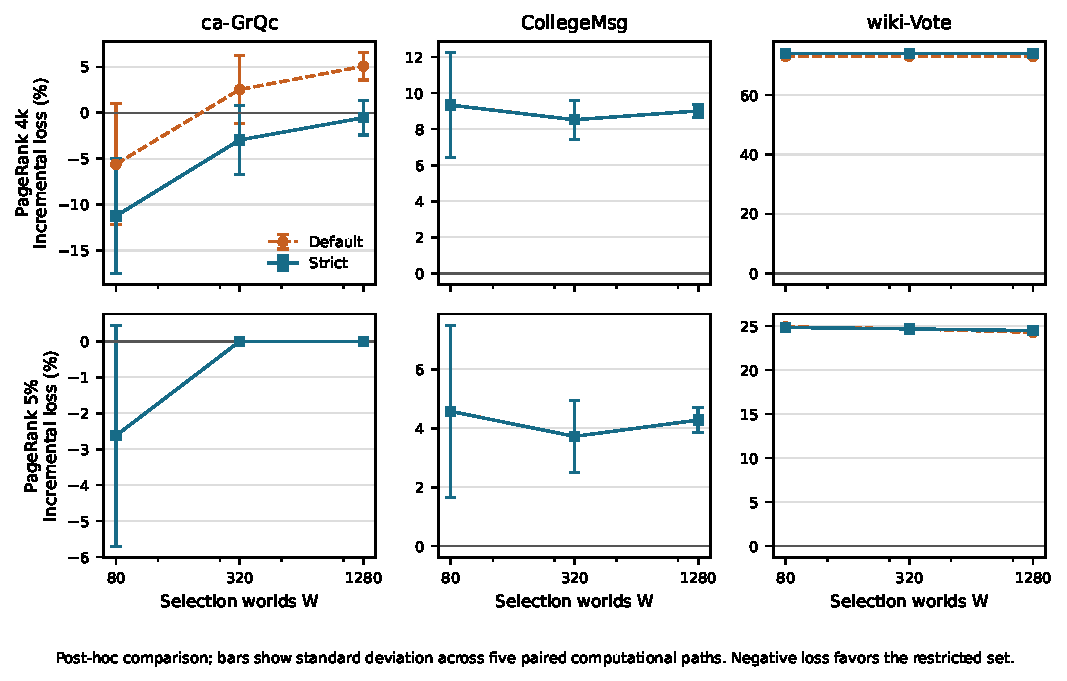
\includegraphics[width=\linewidth]{Fig4.pdf}
\caption{Budget and ranking precision have distinct effects on candidate-restriction quality. Points are mean incremental losses over five paired paths; bars are path standard deviations. The plotted labels Default and Strict denote tolerances $10^{-6}$ and $10^{-12}$; candidate membership is unchanged between $10^{-12}$ and $10^{-14}$. Negative loss favors the restricted set. The ca-GrQc default reversal disappears with the tighter PageRank tolerance, while the directed-network losses persist. This is a post-hoc paired sensitivity analysis.}\label{fig:precision-budget}
\end{figure}

\subsection{Changing the reference set does not determine the spread change}
Figure~\ref{fig:transitions} compares reference-set changes with independent utility changes. From $W=320$ to 1280, all five ca-GrQc sets change, but their mean gain is 0.12720 nodes; individual differences range from $-0.0266$ to $+0.2411$. CollegeMsg changes one set and gains 0.05336 nodes averaged across all five paths. wiki-Vote changes no final sets and has exactly zero paired gain, although some ordered sequences change.

Of the six changed sets, four have positive pointwise 95\% conditional Monte Carlo intervals; two ca-GrQc intervals include zero. The nine unchanged sets have identical evaluation vectors.

In the historical step-coupled comparison from $W=1280$ to 5120, 16/40 sets changed while the mean high-minus-low budget gain was 0.01111 nodes (range $-0.0383$ to $+0.1180$). Historical fixed-edge references also change: from $W=320$ to 1280, 29/40 sets changed, with mean high-minus-low budget gain 0.061845 nodes (range $-0.0110$ to $+0.2572$). Each transition uses a shared evaluation family within its own coupling. Because the two budget intervals differ, their mean gains do not estimate a coupling effect.
\begin{figure}[t]
\centering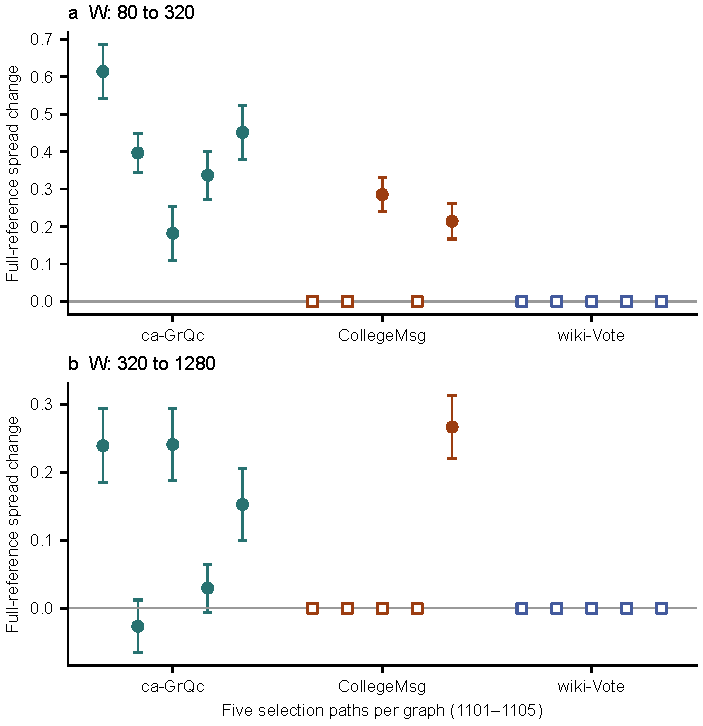
\includegraphics[width=\linewidth]{Fig2.pdf}
\caption{Reference-set changes and independent spread changes. Filled circles denote changed final sets; hollow squares denote unchanged sets. Paths 1101--1105 run from left to right within each graph. Bars are unadjusted 95\% conditional Monte Carlo intervals from 10,000 paired worlds. Panel-specific vertical scales reveal small changes; the intervals condition on selected sets and do not describe variation across networks.}\label{fig:transitions}
\end{figure}

\subsection{Ranking agreement depends on coverage and network context}
At $W=1280$, Degree-4k reproduces every full-candidate reference trajectory across the three external graphs using only 20 candidates (Table~\ref{tab:primary}). Default PageRank-4k matches none and incurs mean incremental losses of \GrqcPRLoss{}\%, \CollegePRLoss{}\% and \WikiPRLoss{}\% on ca-GrQc, CollegeMsg and wiki-Vote. The historical extension showed much broader PageRank agreement: 40/40 trajectories at $W=5120$, compared with 39/40 for degree. The external results therefore limit transfer of the contact-graph ranking result.
\begin{table}[htbp]
\caption{External results at $W=1280$ (five paths). Degree-4k and PageRank-4k (PR) use 20-node pools; PR uses default tolerance. Full incremental spread is total spread minus $k=5$. PR gap is restricted minus full mean spread; loss is relative to full incremental spread. Degree agreement counts identical ordered trajectories.}\label{tab:primary}
\begin{tabular}{lrrrr}
\toprule
Graph & \shortstack{Full incremental\\spread (nodes)} & \shortstack{PR gap\\(nodes)} & \shortstack{PR loss\\(\%)} & \shortstack{Degree\\agreement} \\
\midrule
ca-GrQc & 4.934 & -0.25082 & 5.07 & 5/5 \\
CollegeMsg & 10.072 & -0.90780 & 9.01 & 5/5 \\
wiki-Vote & 55.736 & -40.69334 & 73.01 & 5/5 \\
\bottomrule
\end{tabular}
\par\smallskip\footnotesize Agreement is the number of matching trajectories out of five paths.
\end{table}


For the primary comparisons at the highest tested external budget, every default PageRank-4k and within-path random-4k mean difference from full selection is negative, giving unadjusted sign-test $p=.0625$ and within-graph Holm $p=.1875$. Degree-4k differences from full selection are exactly zero. Five paths limit the minimum two-sided sign-test value to .0625; these results establish neither statistical equivalence nor absence of loss. The paired effect sizes, sensitivity controls and complete test results are reported in Online Resource 1.

Increasing the default PageRank pool to 5\% reproduces all five ca-GrQc references at $W=1280$ and reduces CollegeMsg loss from \CollegePRLoss{}\% to \CollegePRfiveLoss{}\%. On wiki-Vote, loss falls from \WikiPRLoss{}\% to \WikiPRfiveLoss{}\%, remaining above one fifth of full-reference incremental spread. Historical-weighted CollegeMsg pools similarly improve from a mean difference of $-0.25224$ nodes at 4k to exact reference reproduction at 5\%. Coverage helps in these comparisons, but its effect differs across networks.

On wiki-Vote, the default PageRank top 20 have mean in-degree 249.75 and out-degree 56.2; the degree top 20 have mean in-degree 70.3 and out-degree 489.25. The PageRank-4k pool contains none of the five full-reference seeds on any $W=1280$ path, and its 5\% pool contains only one. The seed-level illustration and complete coverage comparisons appear in Online Resource 1.

\subsection{Reference-preserving savings under specified timing scopes}
Degree-4k reduces measured selection time by 98.40--99.67\% relative to this implementation's full-candidate reference at $W=1280$, while reproducing all its trajectories (Table~\ref{tab:cost}). Including setup, both world families and independent evaluation gives assembled cost savings of \CollegeDegreeSaving{}--\WikiDegreeSaving{}\%.
\begin{table}[htbp]
\caption{Degree-4k cost at $W=1280$, averaged over five paths. Full and Degree columns give measured selection time. The final column estimates savings including setup, preparation of selection and evaluation worlds, selection and independent evaluation. These assembled warm-process costs exclude imports, JIT compilation, downloads and output writing; they are not direct end-to-end timings.}\label{tab:cost}
\begin{tabular}{lrrrr}
\toprule
Graph & Full (s) & Degree (s) & \shortstack{Selection\\saving (\%)} & \shortstack{Saving including\\evaluation (\%)} \\
\midrule
ca-GrQc & 23.53 & 0.109 & 99.54 & 92.77 \\
CollegeMsg & 5.89 & 0.094 & 98.40 & 86.59 \\
wiki-Vote & 158.94 & 0.520 & 99.67 & 96.26 \\
\bottomrule
\end{tabular}
\end{table}


At $W=1280$, Degree-4k meets the zero point-estimate loss threshold relative to full selection on every path. Default PageRank-4k meets 10\% on ca-GrQc and CollegeMsg, but fails 20\% on every wiki-Vote path. None of the random-pool path means meets 20\%. Online Resource 1 reports all six frozen thresholds (0, 1, 2.5, 5, 10 and 20\%) and their cost estimates; these are descriptive criteria rather than application-validated tolerances.

\subsection{Parameter and coupling controls delimit the findings}

In the external fixed-edge control at $W=320$, default PageRank-4k minus the fixed-edge full reference has mean spread differences of $-0.16240$, $-0.93417$ and $-40.57597$ nodes on ca-GrQc, CollegeMsg and wiki-Vote. Degree-4k reproduces 1/3, 3/3 and 3/3 corresponding trajectories. The PageRank losses persist under this control, while some reference-agreement outcomes change. Complete control paths and repeated timings are supplied in Online Resource 1.

Across the 160 historical nondefault parameter conditions at $W=320$, Degree-4k and PageRank-4k reproduce 117 and 132 full-reference trajectories, respectively. Weighted-4k minus full selection has 117 negative and 43 positive paired spread differences. These are descriptive counts of repeated computations, not independent success trials.

Under historical fixed-edge sampling at $W=1280$, Degree-4k and PageRank-4k match 38/40 and 40/40 trajectories of the fixed-edge full reference, while Weighted-4k matches 5/40. The supplementary tables retain every graph and setting. These contact-graph controls do not test the joint effect of the tighter PageRank tolerance and fixed-edge sampling on the external graphs.
\FloatBarrier

\section{Discussion}
\subsection{What a budget comparison can establish}
The ca-GrQc result changes the interpretation of an apparent budget effect. At default PageRank tolerance, increasing the reference budget changes the restricted method's mean comparison from a gain to a loss. Tightening tolerance exchanges two pool members and removes that pattern, although increasing $W$ still changes selected sets. Thus, the default reversal is not evidence for a budget effect that is independent of ranking precision. The candidate cutoff makes numerical ranking differences relevant to seed eligibility. Pool agreement at $10^{-12}$ and $10^{-14}$ checks membership stability at the tested tolerances, without certifying an exact ranking. Losses persist on CollegeMsg and wiki-Vote, so this explanation does not account for every unfavorable PageRank comparison.

StaticGreedy already makes reuse of sampled realizations central to a consistent finite objective \cite{ref8}. Our fixed-edge control follows the same coverage principle, whereas the primary step-indexed coupling can produce a nonmonotone finite objective. This distinction concerns the sampled construction and does not contradict the expected-spread result of Kempe et al. \cite{ref1}. The additional issue identified here occurs before selection: numerical tolerance can change which vertices enter a truncated pool. Shared worlds control the comparison between eligible sets, but do not remove this dependence on pool construction.

\subsection{From seed agreement to a quality--cost judgment}
Benchmarking work examines influence-maximization quality together with computational cost \cite{ref16}. Our paired comparisons add a distinction between preserving a reference's seeds and preserving its independently evaluated utility. A changed trajectory may end at the same set, which gives the same evaluation vector under shared simulation worlds. When sets differ, paired evaluation measures the sign, magnitude and conditional uncertainty of their utility difference. The external ca-GrQc mean change of 0.12720 nodes and the historical step-coupled mean change of 0.01111 nodes illustrate distinct budget transitions. Neither value defines an application-specific equivalence margin.

This distinction changes how a reported speed saving should be read. The degree-pool results identify computation saved while preserving the tested reference. The PageRank results require the corresponding utility loss to be considered alongside that saving. Candidate fraction, ranking tolerance and reference budget specify the quality comparison; included timing stages specify the cost comparison. These observations complement solver-efficiency research by clarifying the measured trade-off, without providing a runtime comparison against CELF or IMM.

\subsection{Network direction and transfer of ranking results}
The wiki-Vote observations are consistent with a mismatch between incoming importance and outgoing propagation. The PageRank pool emphasizes vertices with many incoming links, while diffusion in this study follows outgoing arcs. Direction was not experimentally reversed, so the diagnostic does not isolate a causal mechanism. Network structure, candidate coverage and the propagation setting remain relevant to the observed loss. The broader distinction between a simulated objective and an empirical influence model also matters \cite{ref15}. Agreement on contact graphs cannot by itself establish that a ranking will preserve utility on differently directed networks. The increase in PageRank coverage improves the measured comparison, but does not eliminate the wiki-Vote loss.

\subsection{Scope, limitations and next tests}
The external evidence covers three selected networks under $k=5$, $p=.01$, $h=3$ and selection budgets up to 1280. Historical contact graphs also probe $p$, $h$, coupling and $k$, but their local parameter changes are not a full factorial design and do not establish sensitivity on the larger directed graphs. At historical $k=20$, the 4k pool contains all 75 Kenya vertices and 80/91 invs2013 vertices; Kenya agreement is a full-pool identity check. The historical fixed-edge controls also do not validate the external tighter-tolerance PageRank results under fixed-edge sampling.

Paths repeat computations on a fixed graph, and the networks are not a probability sample of social systems. Each synthetic control uses one fixed graph, so repeated paths do not add graph instances. Conditional Monte Carlo uncertainty concerns fixed selected sets; path variation concerns the computational repetitions, not cross-network generalization. Observed relations provide topology, not calibrated causal diffusion. The direction diagnostic is consistent with the measured wiki-Vote loss but does not establish a causal explanation.

Reference agreement establishes neither optimality with respect to expected spread nor convergence as the world budget increases. The cost comparison uses this implementation's exhaustive full-candidate reference, not CELF or IMM. Measured selection costs and assembled costs including independent evaluation answer different deployment questions. The latter exclude cold-start overhead and are not direct end-to-end timings; tighter-tolerance PageRank is assessed for quality only.

\paragraph{Next tests.} Two targeted studies follow from these limits. A joint tolerance--coupling control on the external networks would test whether the precision-sensitive interpretation persists with fixed-edge worlds. A direction intervention, with the remaining settings held constant, would help distinguish the proposed directional explanation from other structural differences. Broader external probability and horizon settings are also needed before extending the contact-graph sensitivity results. These are open tests, not outcomes established by the current data.

\section{Conclusion}
Candidate-restriction quality must be interpreted relative to both a sampled reference and a numerically constructed candidate pool. Through paired controls and independent evaluation, this study separates numerical sensitivity, seed agreement and utility retention. On ca-GrQc, tightening PageRank tolerance removes the apparent budget-induced quality reversal, while budget-dependent seed changes remain. Across the external sample, Degree-4k preserves the tested $W=1280$ trajectories at lower measured selection cost, while PageRank outcomes depend on precision, coverage and network context. These findings make the basis of a measured quality--cost trade-off explicit. Their scope is the studied networks and settings; matching a finite reference does not establish expected-spread optimality. Joint precision--coupling controls and direction interventions are the next tests of the interpretation beyond the present comparisons.

\paragraph{Supplementary information.} Online Resource 1 contains the external result matrix, precision and direction diagnostics, loss--cost curves, and separate historical coverage, parameter, coupling and secondary-control tables with reproducibility details.
\section*{Statements and Declarations}
\paragraph{Funding.} This work was supported by a provincial undergraduate innovation and entrepreneurship training project.
\paragraph{Competing interests.} The authors declare that they have no competing interests.
\paragraph{Author contributions.} Jiayue Sun: conceptualization, methodology, software, validation, formal analysis, investigation, data curation, visualization, and writing---original draft. Binbin Yong: supervision, methodology, project administration, and writing---review and editing. Junjie An: software, data curation, and writing---review and editing. Tianyu Bo: validation, visualization, and writing---review and editing. Shuai Li: formal analysis, validation, and writing---review and editing. All authors read and approved the final manuscript and agreed to its submission to \textit{Computing}.
\paragraph{Data availability.} The third-party datasets are available from the cited providers under their access terms and are not redistributed. Source records, expected SHA-256 hashes and preprocessing instructions accompany the submission.
\paragraph{Code availability.} Frozen source snapshots, configurations, validators, analysis scripts, condition-level outputs and figure-source tables are supplied with the submission for editorial and peer-review access.
\begin{thebibliography}{99}
\bibitem{ref1} Kempe D, Kleinberg J, Tardos É (2003) Maximizing the spread of influence through a social network. In: ACM SIGKDD, pp 137--146. \url{https://doi.org/10.1145/956750.956769}

\bibitem{ref7} Leskovec J, Krause A, Guestrin C, Faloutsos C, VanBriesen J, Glance N (2007) Cost-effective outbreak detection in networks. In: KDD, pp 420--429. \url{https://doi.org/10.1145/1281192.1281239}

\bibitem{ref8} Cheng S, Shen H, Huang J, Zhang G, Cheng X (2013) StaticGreedy: solving the scalability-accuracy dilemma in influence maximization. In: CIKM, pp 509--518. \url{https://doi.org/10.1145/2505515.2505541}

\bibitem{ref2} Tang Y, Shi Y, Xiao X (2015) Influence maximization in near-linear time: a martingale approach. In: ACM SIGMOD, pp 1539--1554. \url{https://doi.org/10.1145/2723372.2723734}

\bibitem{ref12} Rui X, Yang X, Fan J, Wang Z (2020) A neighbour scale fixed approach for influence maximization in social networks. Computing 102:427--449. \url{https://doi.org/10.1007/s00607-019-00778-5}

\bibitem{ref13} Fan C, Wang Z, Zhang J, Zhao J, Rui X (2024) Influence maximization in social networks based on discrete harris hawks optimization algorithm. Computing 106:327--351. \url{https://doi.org/10.1007/s00607-023-01207-4}

\bibitem{ref19} Ko J, Kim S, Lee K, et al. (2025) Inductive influence estimation and maximization over unseen social networks under two diffusion models. Data Mining and Knowledge Discovery 39:55. \url{https://doi.org/10.1007/s10618-025-01137-z}

\bibitem{ref9} Li Y, Fan J, Wang Y, Tan K-L (2018) Influence maximization on social graphs: a survey. IEEE Transactions on Knowledge and Data Engineering 30:1852--1872. \url{https://doi.org/10.1109/TKDE.2018.2807843}

\bibitem{ref16} Arora A, Galhotra S, Ranu S (2017) Debunking the myths of influence maximization: an in-depth benchmarking study. In: SIGMOD, pp 651--666. \url{https://doi.org/10.1145/3035918.3035924}

\bibitem{ref11} Yanchenko E, Murata T, Holme P (2024) Influence maximization on temporal networks: a review. Applied Network Science 9:16. \url{https://doi.org/10.1007/s41109-024-00625-3}

\bibitem{ref15} Aral S, Dhillon PS (2018) Social influence maximization under empirical influence models. Nature Human Behaviour 2:375--382. \url{https://doi.org/10.1038/s41562-018-0346-z}

\bibitem{networkxpr} NetworkX developers (2025) PageRank, NetworkX 3.5 documentation. \url{https://networkx.org/documentation/networkx-3.5/reference/algorithms/generated/networkx.algorithms.link_analysis.pagerank_alg.pagerank.html}. Accessed 15 October 2026

\bibitem{snap} Leskovec J, Krevl A (2014) SNAP datasets: Stanford large network dataset collection. \url{https://snap.stanford.edu/data}. Accessed 15 October 2026

\bibitem{college} Panzarasa P, Opsahl T, Carley KM (2009) Patterns and dynamics of users' behavior and interaction: Network analysis of an online community. Journal of the American Society for Information Science and Technology 60:911--932. \url{https://doi.org/10.1002/asi.21015}

\bibitem{grqc} Leskovec J, Kleinberg J, Faloutsos C (2007) Graph evolution: densification and shrinking diameters. ACM Transactions on Knowledge Discovery from Data 1(1):2. \url{https://doi.org/10.1145/1217299.1217301}

\bibitem{signed} Leskovec J, Huttenlocher D, Kleinberg J (2010) Signed networks in social media. In: CHI, pp 1361--1370. \url{https://doi.org/10.1145/1753326.1753532}

\bibitem{links} Leskovec J, Huttenlocher D, Kleinberg J (2010) Predicting positive and negative links in online social networks. In: WWW, pp 641--650. \url{https://doi.org/10.1145/1772690.1772756}

\bibitem{ref3} Génois M, Vestergaard CL, Fournet J, Panisson A, Bonmarin I, Barrat A (2015) Data on face-to-face contacts in an office building suggest a low-cost vaccination strategy based on community linkers. Network Science 3:326--347. \url{https://doi.org/10.1017/nws.2015.10}

\bibitem{ref4} Génois M, Barrat A (2018) Can co-location be used as a proxy for face-to-face contacts? EPJ Data Science 7:11. \url{https://doi.org/10.1140/epjds/s13688-018-0140-1}

\bibitem{ref5} Cattuto C, Van den Broeck W, Barrat A, Colizza V, Pinton J-F, Vespignani A (2010) Dynamics of person-to-person interactions from distributed RFID sensor networks. PLoS ONE 5:e11596. \url{https://doi.org/10.1371/journal.pone.0011596}

\bibitem{ref6} Kiti MC, Tizzoni M, Kinyanjui TM, et al. (2016) Quantifying social contacts in a household setting of rural Kenya using wearable proximity sensors. EPJ Data Science 5:21. \url{https://doi.org/10.1140/epjds/s13688-016-0084-2}

\bibitem{ref17} Barabasi A-L, Albert R (1999) Emergence of scaling in random networks. Science 286:509--512. \url{https://doi.org/10.1126/science.286.5439.509}

\bibitem{ref18} Holland PW, Laskey KB, Leinhardt S (1983) Stochastic blockmodels: first steps. Social Networks 5:109--137. \url{https://doi.org/10.1016/0378-8733(83)90021-7}
\end{thebibliography}

\end{document}
